\begin{frame}[plain]
  \begin{center}
    \vspace{2em}
    {\LARGE\textbf{Vision-Language Models}}

    \vspace{2.5em}
    {\scriptsize Slides in this section adapted from D. Kiela, ``Multimodal Deep Learning (with an NLP focus)'',\\
    guest lecture, Stanford CS224n, Winter 2023.}
  \end{center}
\end{frame}

\begin{frame}{CLIP: Contrastive Language-Image Pretraining}
  \begin{itemize}
    \item[] \textbf{Developed by OpenAI (Radford et al., ICML 2021)}
    \vspace{0.6em}
    \item Trained on 400M (image, text) pairs scraped from the web
    \item \textbf{Contrastive objective:} for a batch of $N$ pairs, score all $N \times N$ image-text
      combinations by cosine similarity, then train so that each image ranks its own caption above
      the other $N-1$ captions, and each caption ranks its own image above the other $N-1$ images
    \item No labels are needed: the caption a human already wrote is the supervision
  \end{itemize}

  \vspace{0.7em}
  \textbf{Use cases:}
  \begin{itemize}
    \item Zero-shot classification
    \item Semantic similarity
    \item Prompt-based image querying
  \end{itemize}
\end{frame}

\begin{frame}{CLIP: Architecture and Reference}
  \textbf{Architecture:}
  \begin{itemize}
    \item[{\color{red}\textbullet}] ResNet or ViT for images
    \item[{\color{red}\textbullet}] Transformer for text
    \item[{\color{red}\textbullet}] Symmetric cross-entropy over temperature-scaled cosine similarities
      (the InfoNCE loss); cosine similarity is the score, not the loss
  \end{itemize}

  \vspace{1em}
  \textbf{Paper:}
  \href{https://arxiv.org/abs/2103.00020}{\colorbox{yellow!20}{Learning Transferable Visual Models From Natural Language Supervision}}
  \hspace{0.5em}
  {\scriptsize\ttfamily https://arxiv.org/abs/2103.00020}
\end{frame}

\begin{frame}{CLIP (Radford et al. 2021)}
  \begin{itemize}
    \item \textbf{Contrastive learning at scale: Transformer encoders trained on web-scraped image-text pairs.}
  \end{itemize}
  \vspace{0.5em}
  \begin{figure}
    \centering
    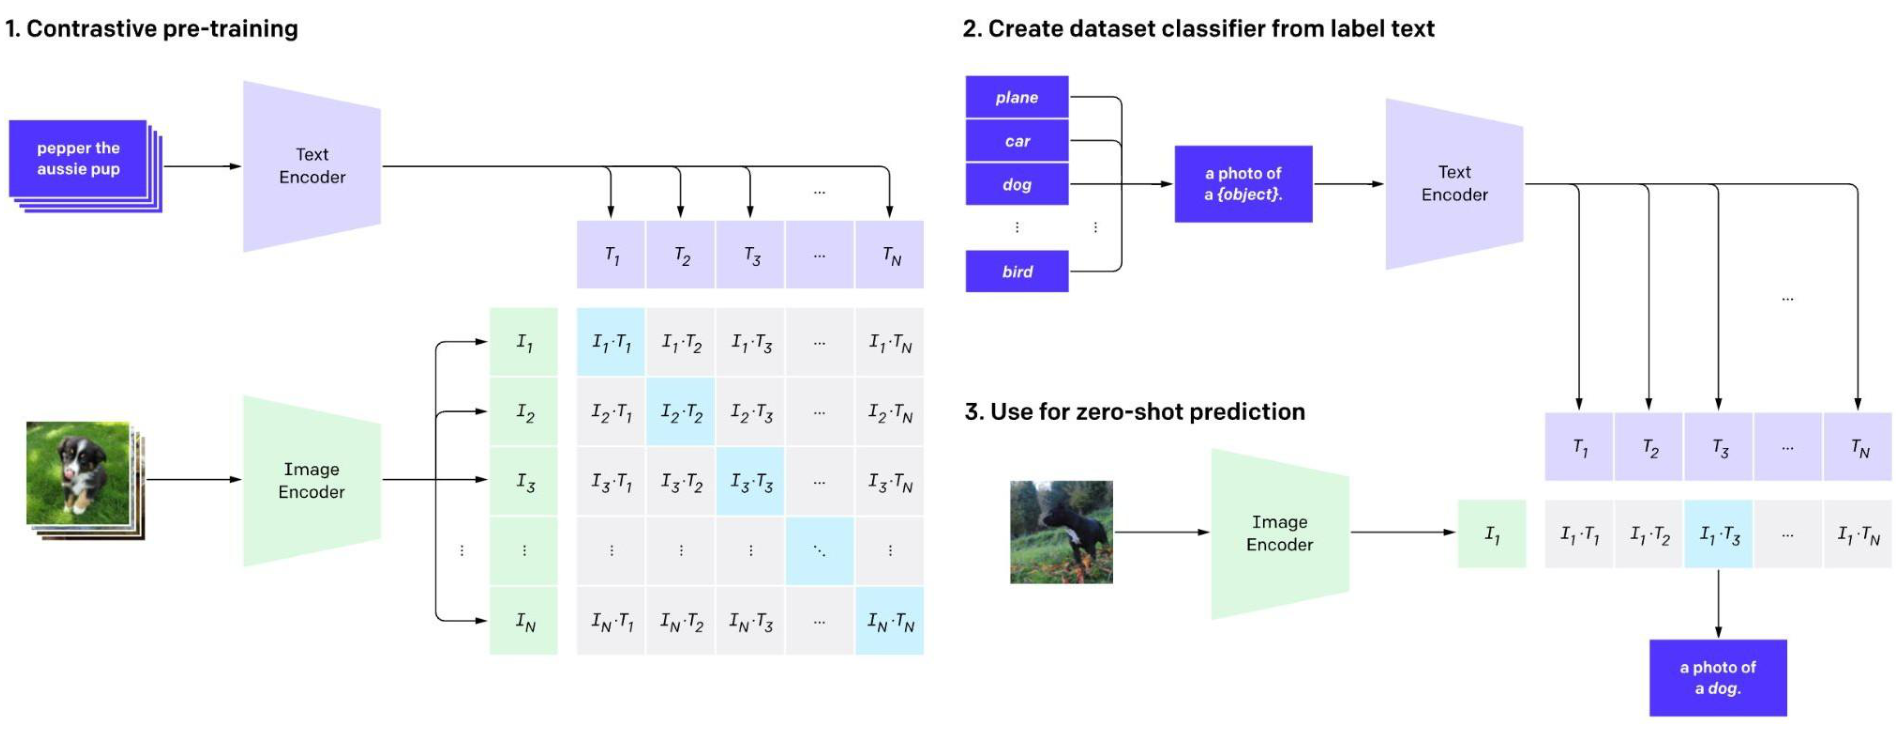
\includegraphics[width=0.9\textwidth, height=0.72\textheight, keepaspectratio]{images/multimodal-nlp-agentic-ai/multimodal_clip_contrastive_pretraining.png}
    \caption*{\scriptsize Source: Radford et al., ``Learning Transferable Visual Models From Natural Language Supervision'', ICML 2021, Figure~1.}
  \end{figure}
\end{frame}

\begin{frame}{CLIP Robustness}
  \begin{columns}[T,onlytextwidth]
    \column{0.42\textwidth}
      \begin{itemize}
        \item A supervised ImageNet model and zero-shot CLIP tie on ImageNet itself.
        \item On the same object photographed differently, sketched, rendered, or chosen adversarially, the supervised model collapses and CLIP does not.
        \item Matching accuracy on the benchmark does not imply matching accuracy on the concept.
      \end{itemize}
    \column{0.56\textwidth}
      \begin{figure}
        \centering
        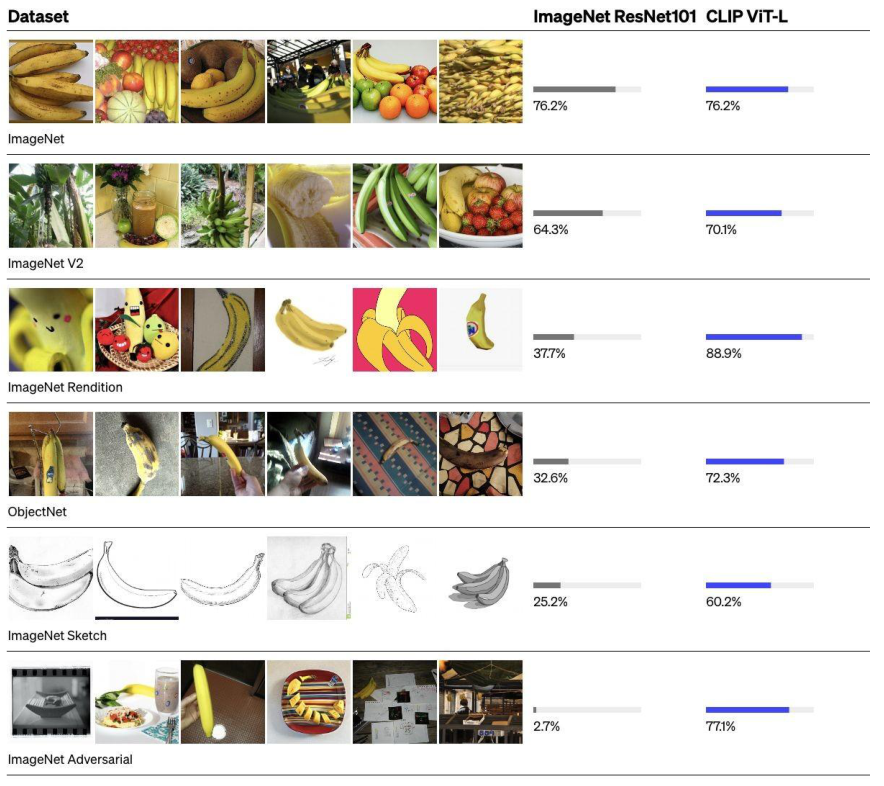
\includegraphics[width=\linewidth, height=0.7\textheight, keepaspectratio]{images/multimodal-nlp-agentic-ai/multimodal_clip_distribution_shift_robustness.png}
        \caption*{\scriptsize Source: Radford et al., ICML 2021, Figure~13 (right panel).}
      \end{figure}
  \end{columns}
\end{frame}

\begin{frame}{VisualBERT: Overview}
  \begin{itemize}
    \item[{\color{red}\textbullet}] \textbf{Joint Transformer-based model:} one stack of Transformer layers
      attends over image regions and text together.
    \item[{\color{red}\textbullet}] \textbf{Early fusion:} region features from a frozen object detector
      (Faster R-CNN trained on Visual Genome) enter as unordered input tokens beside the text tokens.
    \item[{\color{red}\textbullet}] \textbf{Pretraining objectives:}
    \begin{itemize}
      \item Masked language modelling \emph{with the image}: predict masked words using both the
        remaining text and the image regions
      \item Sentence-image prediction: given an image and two captions, decide whether the second one
        describes it
    \end{itemize}
  \end{itemize}
\end{frame}

\begin{frame}{VisualBERT: Applications and Reference}
  \textbf{Applications:}
  \begin{itemize}
    \item Visual Question Answering (VQA)
    \item Image captioning
    \item Visual commonsense reasoning
  \end{itemize}

  \vspace{0.7em}
  \textbf{Paper:}
  \href{https://arxiv.org/abs/1908.03557}{\colorbox{pink!20}{VisualBERT: A Simple and Performant Baseline for Vision and Language}}
  \hspace{0.5em}
  {\scriptsize\ttfamily https://arxiv.org/abs/1908.03557}
\end{frame}

\begin{frame}{Visual BERTs: VisualBERT}
  \begin{figure}
    \centering
    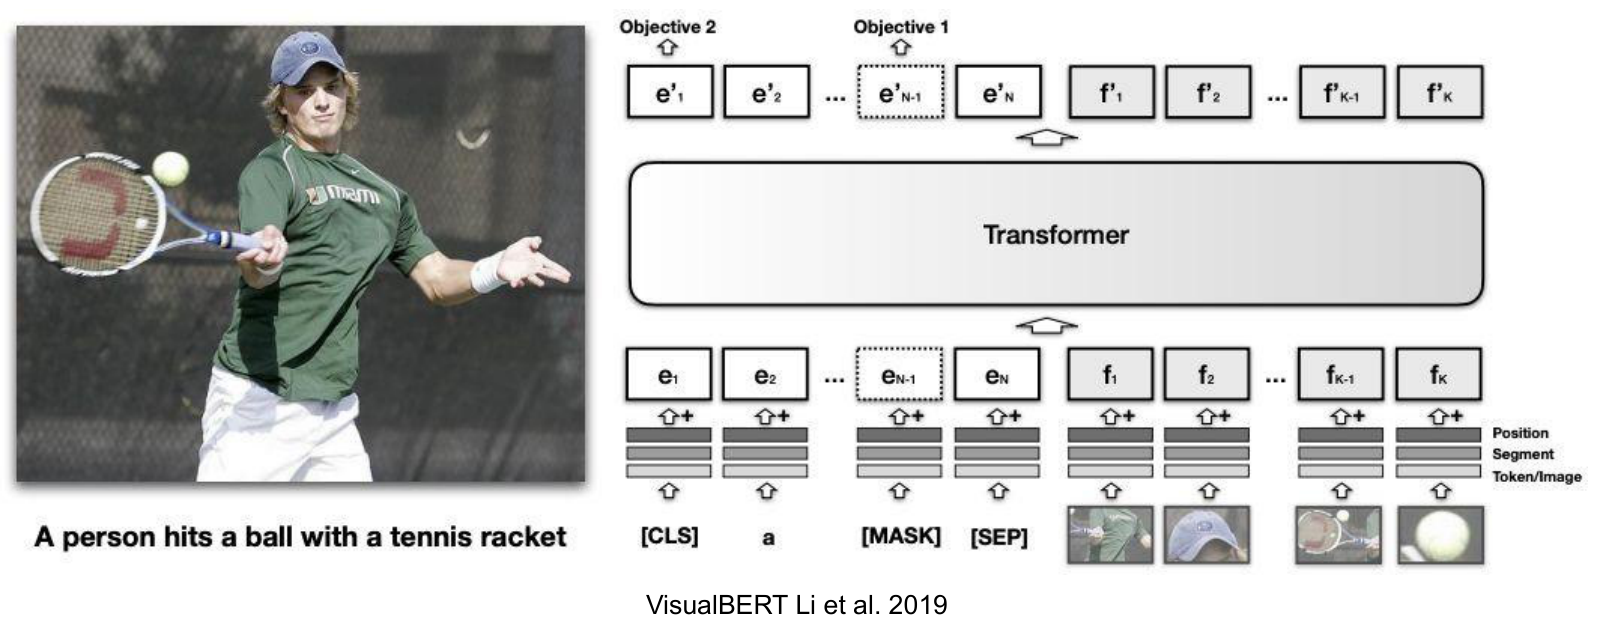
\includegraphics[width=0.98\textwidth, height=0.8\textheight, keepaspectratio]{images/multimodal-nlp-agentic-ai/multimodal_visualbert_architecture.png}
    \caption*{\scriptsize Source: Li et al., ``VisualBERT: A Simple and Performant Baseline for Vision and Language'', \href{https://arxiv.org/abs/1908.03557}{arXiv:1908.03557}, Figure~2.}
  \end{figure}
\end{frame}

\begin{frame}{Visual BERTs: ViLBERT}
  \begin{figure}
    \centering
    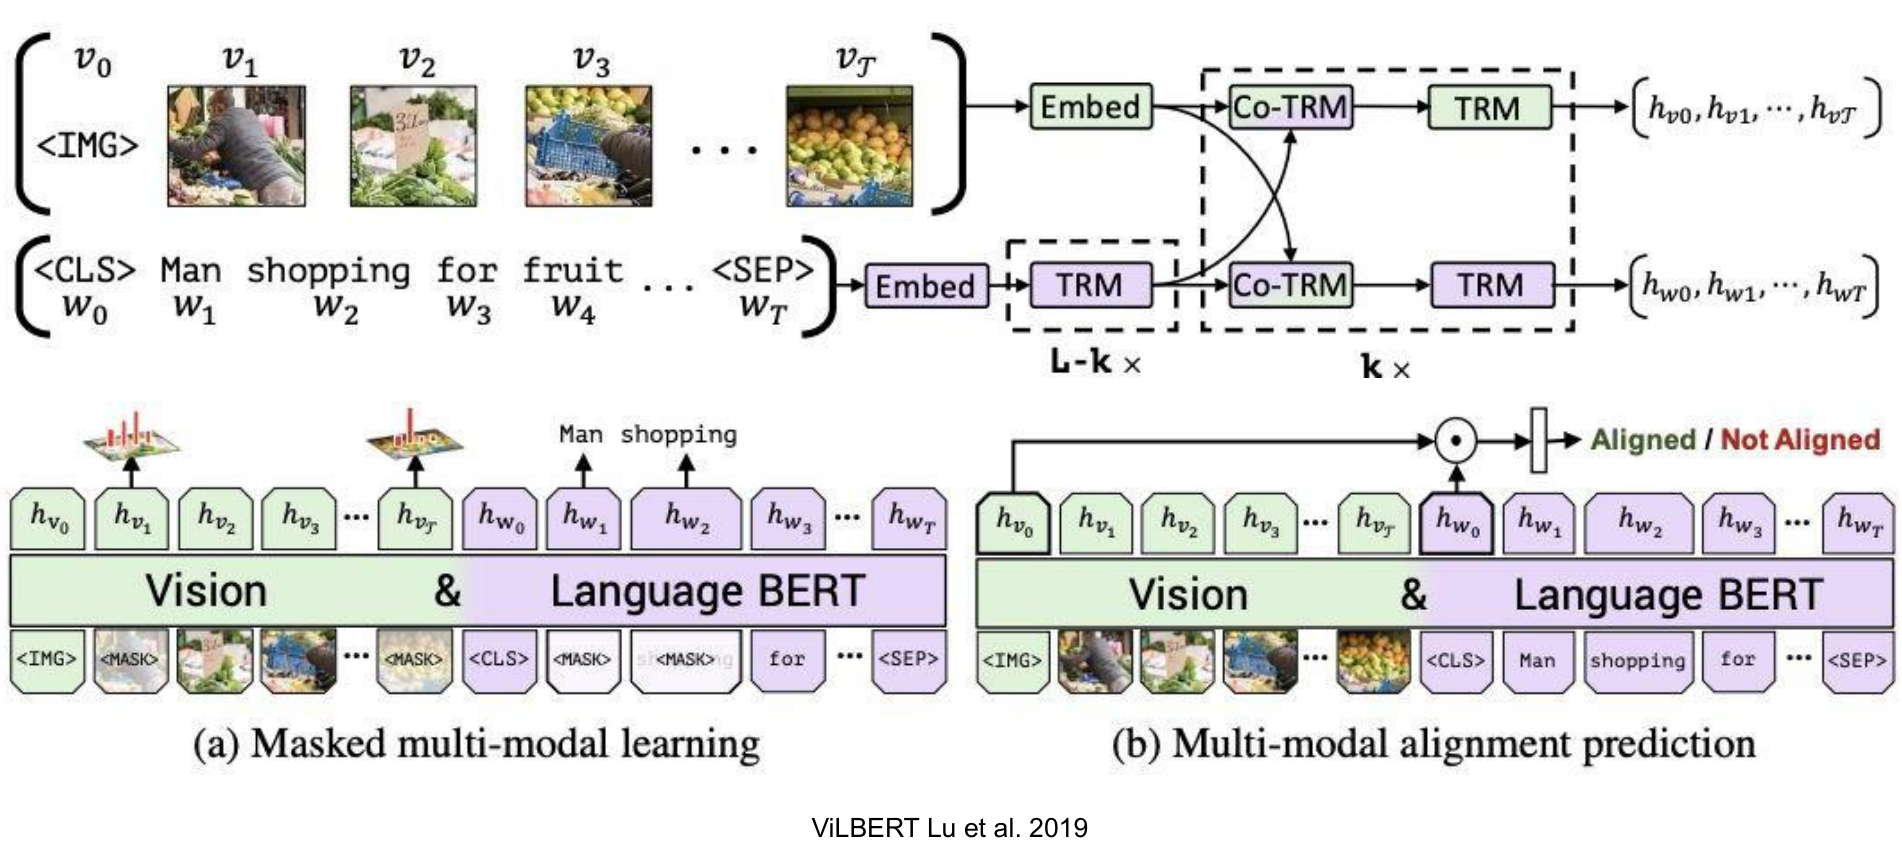
\includegraphics[width=0.98\textwidth, height=0.8\textheight, keepaspectratio]{images/multimodal-nlp-agentic-ai/multimodal_vilbert_architecture.png}
    \caption*{\scriptsize Two streams that stay separate and exchange information through co-attention. Source: Lu et al., ``ViLBERT'', NeurIPS 2019, Figures~1 and~3.}
  \end{figure}
\end{frame}

\begin{frame}{Visual BERTs: LXMERT}
  \begin{figure}
    \centering
    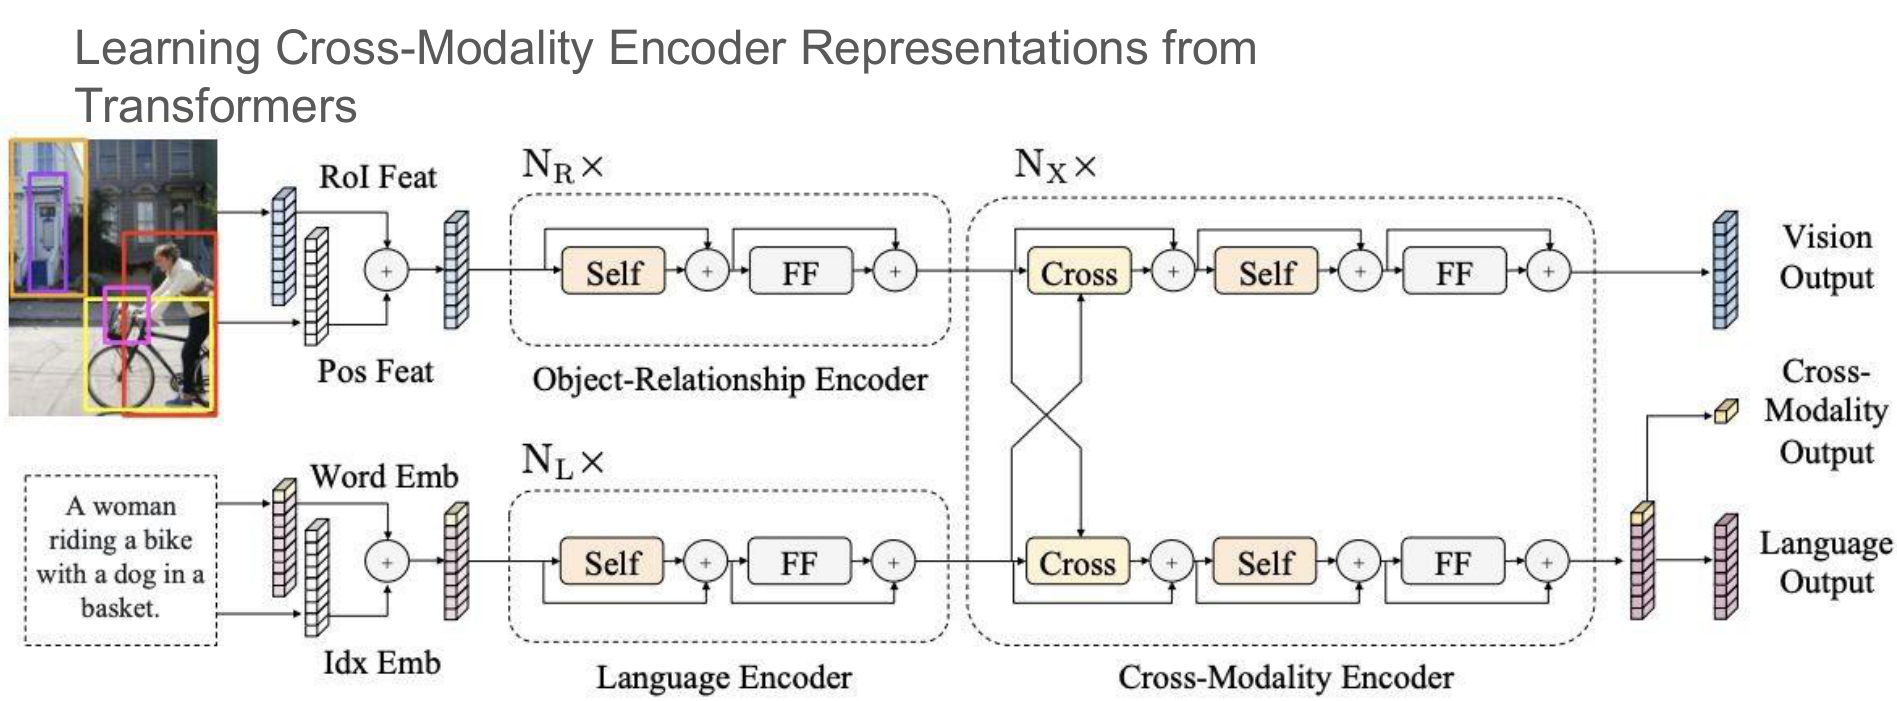
\includegraphics[width=0.92\textwidth, height=0.78\textheight, keepaspectratio]{images/multimodal-nlp-agentic-ai/multimodal_lxmert_architecture.png}
    \caption*{\scriptsize Source: Tan \& Bansal, ``LXMERT: Learning Cross-Modality Encoder Representations from Transformers'', EMNLP 2019, Figure~1.}
  \end{figure}
\end{frame}

\begin{frame}{Visual BERTs: Supervised Multimodal Bitransformers}
  \begin{figure}
    \centering
    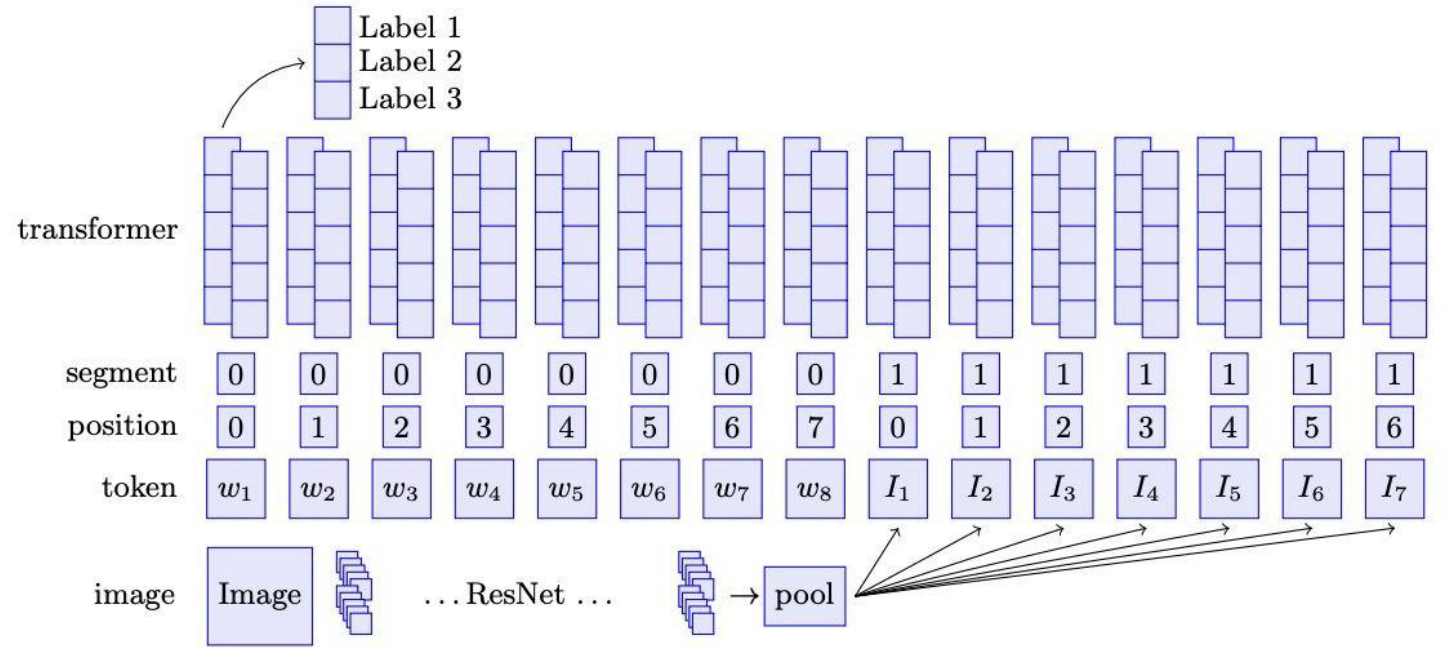
\includegraphics[width=0.98\textwidth, height=0.6\textheight, keepaspectratio]{images/multimodal-nlp-agentic-ai/multimodal_supervised_multimodal_transformer.png}
    \caption*{\scriptsize Source: Kiela et al., ``Supervised Multimodal Bitransformers for Classifying Images and Text'', \href{https://arxiv.org/abs/1909.02950}{arXiv:1909.02950}, Figure~1.}
  \end{figure}
\end{frame}

\begin{frame}{Visual BERTs: Pixel-BERT}
  \begin{figure}
    \centering
    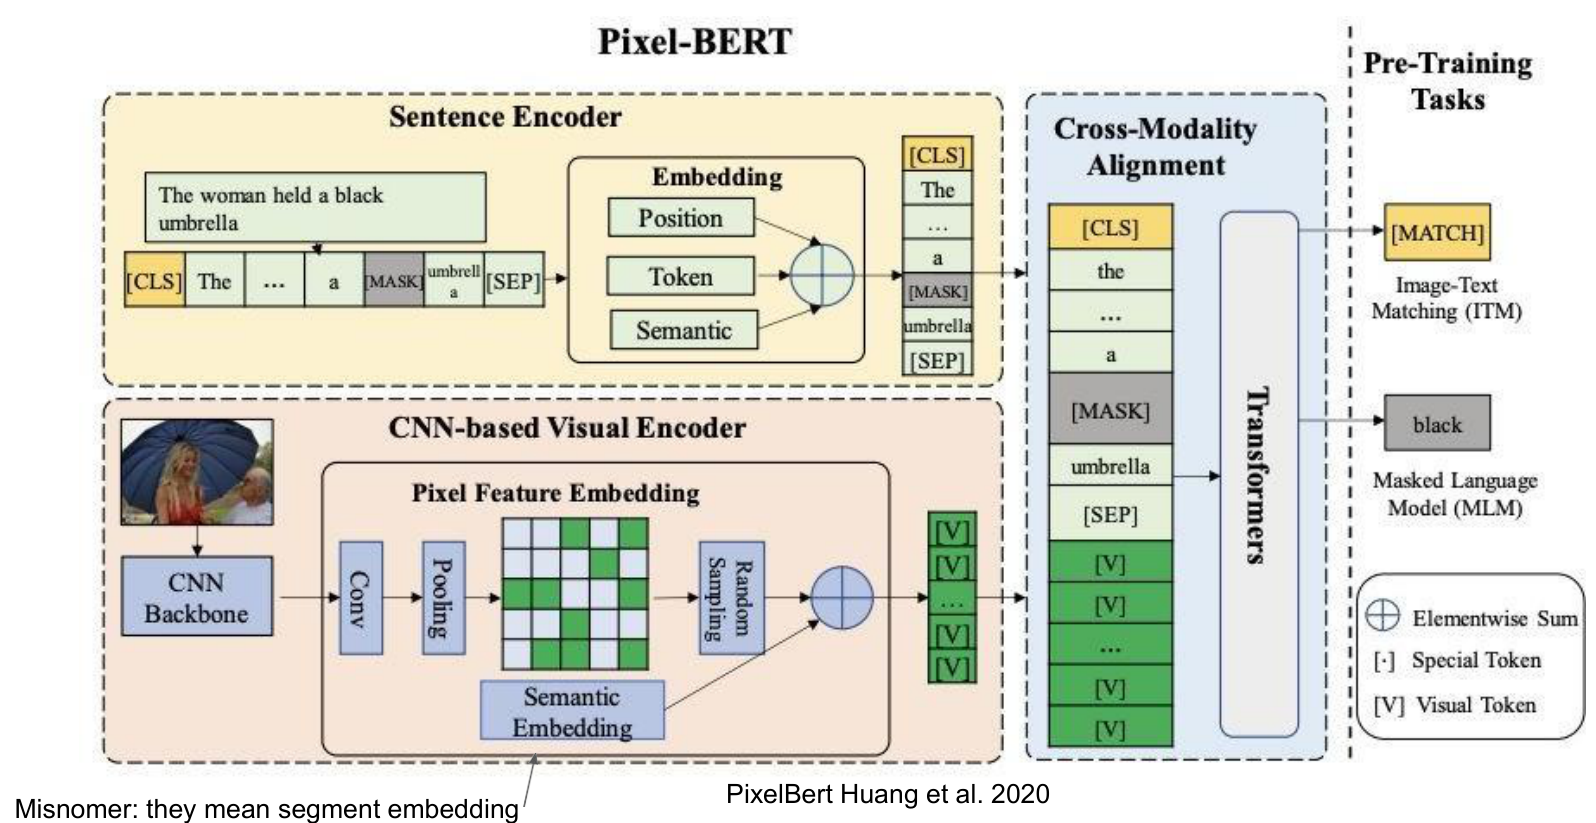
\includegraphics[width=0.98\textwidth, height=0.78\textheight, keepaspectratio]{images/multimodal-nlp-agentic-ai/multimodal_pixelbert_architecture.png}
    \caption*{\scriptsize Region features are dropped: the CNN feeds pixel-level features straight to the Transformer. Source: Huang et al., ``Pixel-BERT'', \href{https://arxiv.org/abs/2004.00849}{arXiv:2004.00849}, Figure~2.}
  \end{figure}
\end{frame}

\begin{frame}{FLAVA (Facebook AI)}
  \begin{itemize}
    \item \textbf{FLAVA = Foundational Language And Vision Alignment}
    \item Handles both unimodal and multimodal tasks
    \item \textbf{Three towers:} vision, language, multimodal
    \item Self-supervised objectives: masked modeling, contrastive learning
  \end{itemize}

  \vspace{0.7em}
  \textbf{Capabilities:}
  \begin{itemize}
    \item Text classification
    \item Image classification
    \item Visual Question Answering (VQA)
    \item Image captioning
  \end{itemize}
  
  \vspace{0.7em}
  \textbf{Paper:}
  \href{https://arxiv.org/abs/2112.04482}{\colorbox{pink!20}{FLAVA: A Foundational Language and Vision Alignment Model}}
  \hspace{0.5em}
  {\scriptsize\ttfamily https://arxiv.org/abs/2112.04482}
\end{frame}

\begin{frame}{FLAVA (Singh et al., 2021)}
  One foundation model spanning vision-and-language, computer vision and NLP. Jointly pre-trained on
  unimodal text (CCNews + BookCorpus), unimodal images (ImageNet-1K), and 70M public paired image-text
  examples (the PMD corpus). All data and models are publicly released.
  \begin{figure}
    \centering
    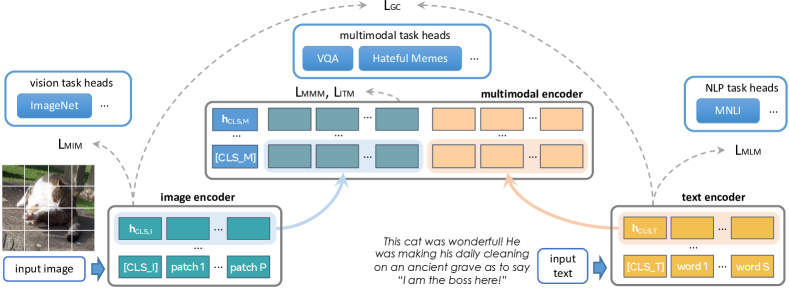
\includegraphics[width=0.98\textwidth, height=0.42\textheight, keepaspectratio]{images/multimodal-nlp-agentic-ai/multimodal_flava_architecture.png}
    \caption*{\scriptsize The three encoders, each with its own losses: masked image modelling, masked
    language modelling, global contrastive between the two towers, and masked multimodal modelling plus
    image-text matching on the joint encoder. Source: Singh et al., CVPR 2022, Figure~2.}
  \end{figure}
\end{frame}

\begin{frame}{From Dual Encoders to Multimodal LLMs}
  \begin{itemize}
    \item[{\color{red}\textbullet}] \textbf{Nomenclature.} An \textbf{LLM} is language-only. A
      \textbf{VLM} (vision-language model) adds a vision encoder so the model can condition on images.
      An \textbf{MLLM} (multimodal LLM) spans several modalities, such as image, video and audio, in one model.
    \item[{\color{red}\textbullet}] \textbf{What the models above can and cannot do.} CLIP scores an
      image against candidate texts; the Visual BERTs classify or answer from a fixed label set. None of
      them writes an answer. A model that has to \emph{describe} an unfamiliar chart, or hold a
      conversation about a photograph, needs a language decoder.
    \item[{\color{red}\textbullet}] \textbf{The shift.} Attach a pretrained vision encoder to a
      pretrained decoder LLM through a small trained module, the \textbf{projector} (also called the
      connector), and train mostly that module. Flamingo (2022), BLIP-2 (2023) and LLaVA (2023)
      established the recipe; Qwen2-VL and GPT-4V-class systems are its production descendants.
    \item[{\color{red}\textbullet}] This is the architecture behind every current multimodal assistant.
      Its variants are compared later in the course.
  \end{itemize}
\end{frame}
